% ctex_test.tex
\documentclass{article}

% Language setting
% Replace `english' with e.g. `spanish' to change the document language
\usepackage[UTF8]{ctex}
\usepackage{setspace}
\usepackage{listings}
\usepackage{xcolor}
\usepackage{listings}
\usepackage[colorlinks,linkcolor=blue]{hyperref}

\lstset{
  backgroundcolor=\color{white},
  basicstyle=\ttfamily\footnotesize,
  breakatwhitespace=false,
  breaklines=true,
  captionpos=b,
  commentstyle=\color{mygreen},
  deletekeywords={...},
  escapeinside={\%*}{*)},
  frame=single,
  keepspaces=true,
  keywordstyle=\color{blue},
  language=Python,
  morekeywords={*,...},
  numbers=left,
  numbersep=5pt,
  numberstyle=\tiny\color{mygray},
  rulecolor=\color{black},
  showspaces=false,
  showstringspaces=false,
  showtabs=false,
  stepnumber=2,
  stringstyle=\color{mymauve},
  tabsize=2,
  title=\lstname
}


% Set page size and margins
% Replace `letterpaper' with `a4paper' for UK/EU standard size
\usepackage[letterpaper,top=2cm,bottom=2cm,left=3cm,right=3cm,marginparwidth=1.75cm]{geometry}

% Useful packages
\usepackage{amsmath}
\usepackage{graphicx}
\usepackage[colorlinks=true, allcolors=blue]{hyperref}

\title{当代人工智能实验报告1}
\author{温兆和 10205501432}

\begin{document}
\maketitle

\section{实验目的}

该任务是一个文本十分类任务。我们需要把\lstinline|./exp1_data/train_data.txt|中的数据分为训练集和验证集,用训练集中的文本和标签对模型进行训练,用验证集检验不同模型、不同超参下的分类效果,并用分类效果最好的模型对\lstinline|./exp1_data/test.txt|中的文本进行分类。

\section{实验环境}
Anaconda3(64-bit)

\textbf{需要安装的工具包有:}
\begin{spacing}{0.5}
\begin{itemize}
\item \lstinline|pandas|
\item \lstinline|numpy|
\item \lstinline|json|
\item \lstinline|gensim|
\item \lstinline|random|
\item \lstinline|string|
\item \lstinline|re|
\item \lstinline|matplotlib|
\item \lstinline|sklearn|
\item \lstinline|scipy|
\item \lstinline|tensorflow|
\item \lstinline|warnings|
\end{itemize}
\end{spacing}

上述大部分工具在Anaconda中无需再次安装。如果有哪个工具包(假设叫\lstinline|X|)需要安装,就直接在Anaconda的.ipynb文件中打开一个新的cell,在里面执行\lstinline|!pip install X|即可,或者也可以执行\lstinline|pip install -r requirements.txt|来安装这些包。
\section{实验步骤}
\subsection{将文本映射成向量}

想要把文本转化为向量,常见的模型有TF-IDF、Word2Vec等。其中,TF-IDF主要是通过统计一个词在文档中出现的频率来衡量其重要性。虽然它更加简单,训练词向量也更加快,但词语不是一个个毫无关联的个体,TF-IDF完全浪费了文本中的上下文信息。此外,如“is”、“the“等词语虽然出现的频率更高,但是它并没有实际的意义。可见,单纯地用词语出现的频率来对文本进行向量化是不合适的。

相比而言,Word2Vec就能更好地利用文本的上下文信息。Word2Vec的本质是一个只有一个隐藏层的神经网络。它的基本思想是:上下文相似的两个词的词向量也应该相似。基于此,本次实验使用Word2Vec进行文本的向量化,以更好地在文本向量中保留文本的上下文含义,从而更好地对文本进行分类。

由于训练集(包括验证集)和测试集中的所有文本总共包含了$50194$个不同的单词,把映射后的文本向量的维度设为$100$已经足够了。设置大小为$10$的窗口长度,来包含十个单词以内的上下文信息。设置最小词频为$5$,保证那些只是偶尔出现的词在训练文本向量的过程中不会被使用到。这将有助于提升模型的准确率。

\begin{lstlisting}
# 训练Word2Vec模型
word2vec = Word2Vec(sentences=corpus, vector_size=100, window=10, min_count=5, sg=1)
word2vec.train(corpus, total_examples=len(corpus), epochs=10)
\end{lstlisting}

\subsection{模型训练与调参}
接下来我们将对不同的模型进行调参,从而让它们都能达到各自的最优性能。在调参过程中,我们将把\lstinline|./exp1_data/train_data.txt|按照$8:2$的比例划分为训练集和验证集,在保证训练集规模的基础上让训练集不要过大而导致模型过拟合。

在真正训练之前,我们还可以对文本向量进行正则化。这可以避免模型在收敛前就达到最大迭代次数。
\begin{lstlisting}
from sklearn.preprocessing import MinMaxScaler
def Standarization(X_train,X_test):
    scaler = MinMaxScaler()
    X_train_scaled = scaler.fit_transform(X_train)
    X_test_scaled = scaler.transform(X_test)
    return X_train_scaled,X_test_scaled
\end{lstlisting}

\subsubsection{逻辑斯蒂回归模型}

为了叙述模型原理时的简便性,我们将从二分类问题推广到多分类问题。在二分类问题中,考虑输入向量 $x$ 和Sigmoid函数 $y=\frac{1}{1+e^{-(w^{T}x+b)}}$ ,则 $y$ 就是样本 $x$ 被分入正类的概率, $1-y$ 就是样本 $x$ 被分入负类的概率。类似地,在多分类问题中,我们也是将样本作为Sigmoid函数的输入,计算其属于各个类别的概率,并取概率最大的类别为其预测类别。

首先,我们寻找正则化力度\lstinline|C|的大致范围。
\begin{lstlisting}
C = []
accu_logreg_C = []
for i in np.arange(0.1, 5, 0.1):
    logreg_para = LogisticRegression(C=i,max_iter=10000)
    logreg_para.fit(X_train,Y_train.values.reshape(-1))
    Y_pred_logreg = logreg_para.predict(X_test)
    C.append(i)
    accu_logreg_C.append(accuracy_score(Y_test, Y_pred_logreg))
plt.plot(C,accu_logreg_C)
plt.xlabel("C")
plt.ylabel("accuracy")
plt.show()
\end{lstlisting}

得到
\begin{figure}[h]
    \centering
    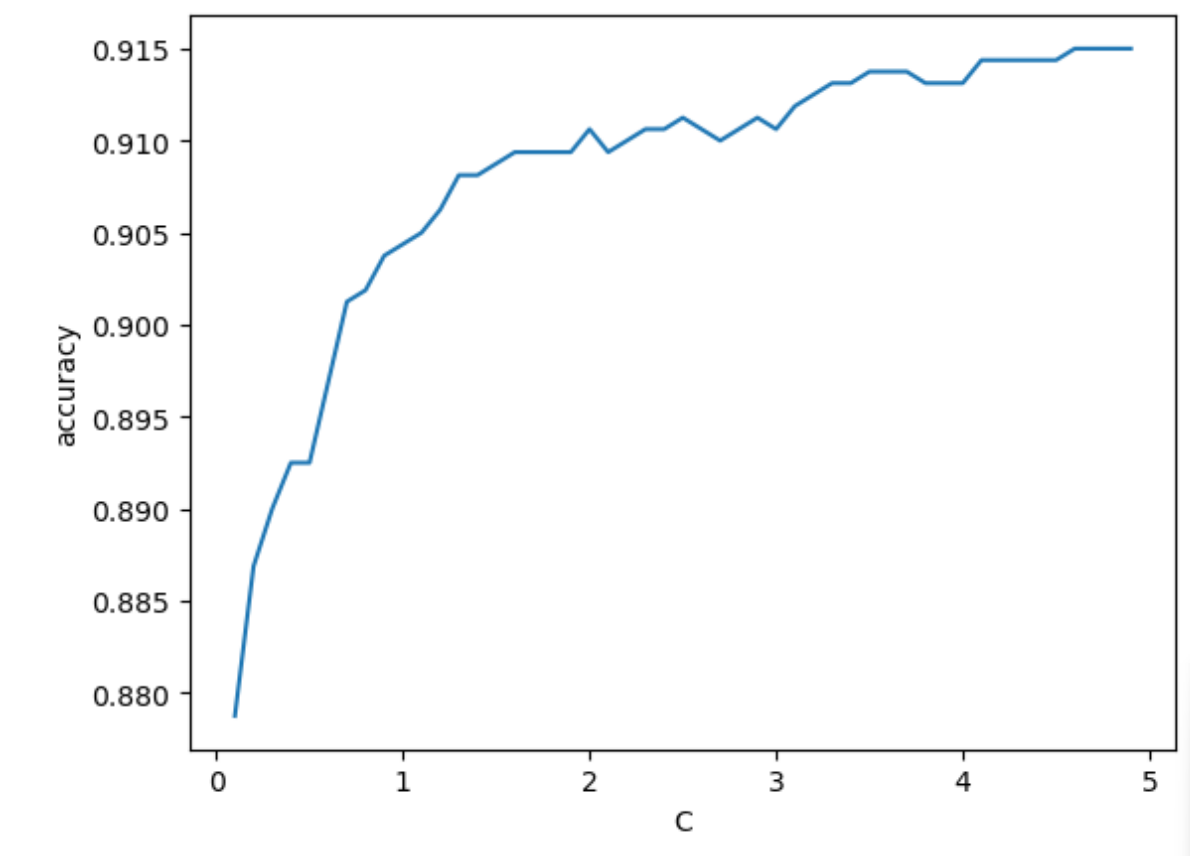
\includegraphics[width=0.5\linewidth]{image1.png}
    %\caption{Enter Caption}
    \label{fig:enter-label}
\end{figure}

可以看到,正则化力度\lstinline|C|在增大到$4$以后,模型的正确率增长放缓。所以,把它的范围设置为$1$—$5$。
再用\lstinline|GridSearchCV()|工具来找出正则化力度\lstinline|C|,各类别样本的权重\lstinline|class_weight|和求解器\lstinline|solver|的最佳参数组合,将这个最优的参数组合设置为模型的超参数并进行五折交叉验证。最大迭代次数\lstinline|max_iter|被设置得尽可能大,从而保证模型一定会收敛。
\begin{lstlisting}
params_logreg = {'C':np.arange(1, 4, 0.5),'class_weight':['balanced', None],'solver':['liblinear','sag','lbfgs','newton-cg']}
logreg_para = LogisticRegression(max_iter=1000)
clf_logreg = GridSearchCV(logreg_para, param_grid=params_logreg, cv=10)
clf_logreg.fit(X_train, Y_train.values.reshape(-1))
logreg_best=clf_logreg.best_params_
X=np.array(df['doc_vector'].tolist())
Y=df.label
kfold = StratifiedKFold(n_splits=5, shuffle=True, random_state=42)
logreg = LogisticRegression(max_iter=1000,**logreg_best)
scores_logreg = cross_val_score(logreg, X, Y, cv=kfold, scoring='accuracy')
print(scores_logreg)
\end{lstlisting}

最后,我们得到五折交叉验证在验证集上的的准确率为
\begin{figure}[h]
    \centering
    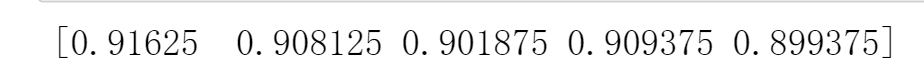
\includegraphics[width=0.5\linewidth]{image2.png}
    %\caption{Enter Caption}
    \label{fig:enter-label}
\end{figure}

\textbf{接下来的几个模型的调参和交叉验证过程与逻辑斯蒂回归模型的过程类似,所以不再详述细节,仅仅展示结果。}

\subsubsection{支持向量机}
支持向量机的思想就是找出各个类别之间的最优超平面,也就是让训练集中各个类别的边缘点离分离超平面距离尽可能大。在分类时,样本点在分离超平面的哪一侧,就认为它属于哪一类。

在支持向量机中,主要有目标函数惩罚系数\lstinline|c|和核函数系数\lstinline|gamma|这两个超参数。我们发现,当\lstinline|c|增大到$0.5$,\lstinline|gamma|增大到$0.5$,模型的准确率不再有显著提升。
\newpage
\begin{figure}[h]
    \lefting
    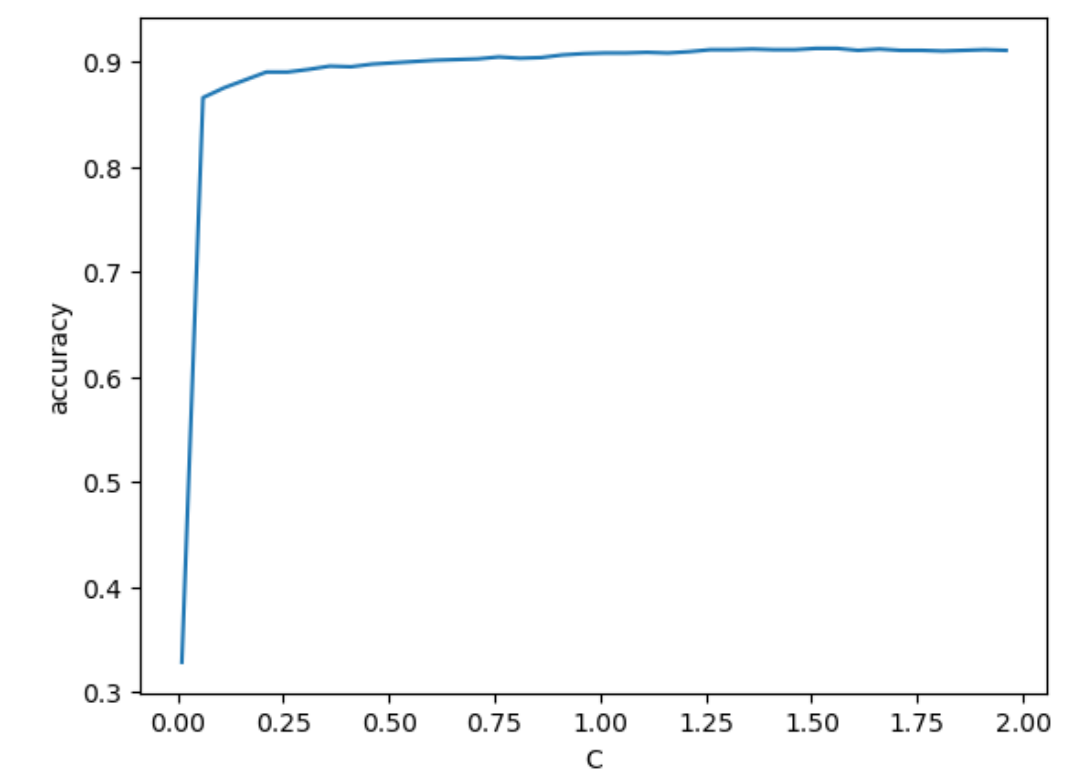
\includegraphics[width=0.5\linewidth]{image3.png}
    %\caption{Enter Caption}
    \label{fig:enter-label}
%\end{figure}\begin{figure}[h]
    \righting
    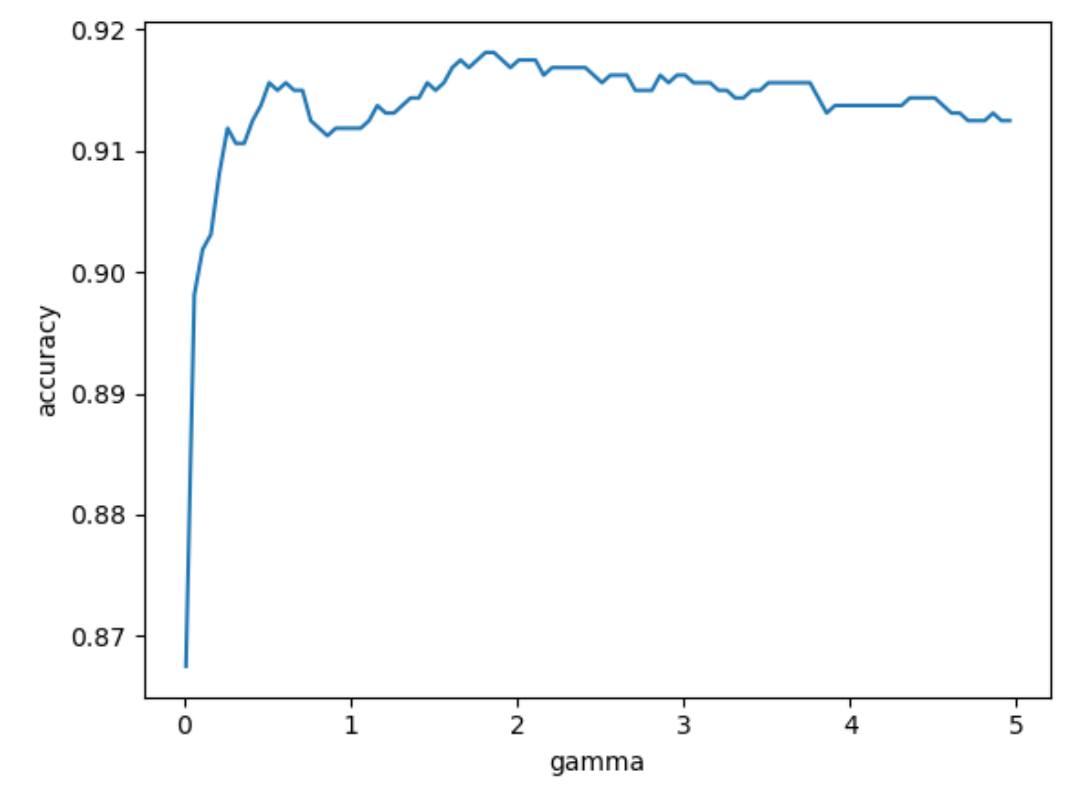
\includegraphics[width=0.5\linewidth]{image4.png}
    %\caption{Enter Caption}
    \label{fig:enter-label}
\end{figure}

所以,我们把\lstinline|c|的范围设置为$0.5$—$2$,\lstinline|gamma|的范围设置为$0.5$—$3$,并找出最优的参数组合。最终,这个最优超参数组合在验证集上的结果是
\begin{figure}[h]
    \centering
    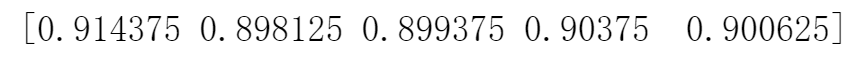
\includegraphics[width=0.5\linewidth]{image5.png}
    %\caption{Enter Caption}
    \label{fig:enter-label}
\end{figure}

\subsubsection{决策树}
决策树是一个很形象的名字,它的基本原理就是构建一棵树,树上的每个节点就代表着一个属性,节点下面的每一个箭头都代表着该属性在不同取值下我们做出的选择,要么指向下一个节点(也就是我们要判断的下一个属性),要么指向某一个分类的结果。

决策树中有这么几个重要的超参数:树的最大深度\lstinline|max_depth|、分割内部节点所需的最小样本数\lstinline|min_samples_split|和叶子节点上的最小样本数\lstinline|min_samples_leaf|。划分标准\lstinline|criterion|使用默认的选项“基尼系数”。

通过实验,我们发现最大深度\lstinline|max_depth|增大到$5$之后模型的准确率不再增长,\lstinline|min_samples_split|和\lstinline|min_samples_leaf|分别控制在$15$和$6$以内模型的分类效果更好。
\begin{figure}[h]
    \lefting
    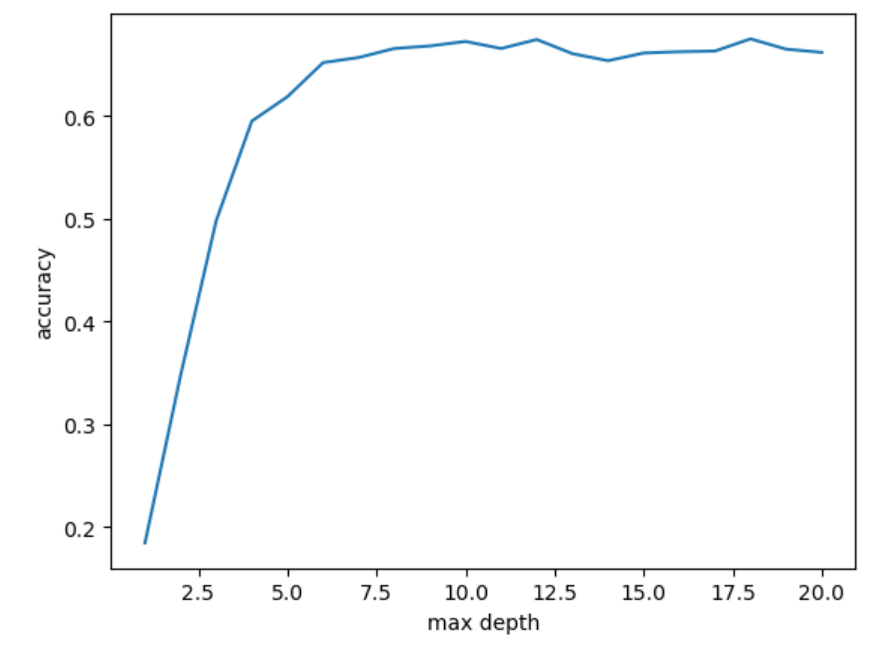
\includegraphics[width=0.3\linewidth]{image6.png}
    %\caption{Enter Caption}
    \label{fig:enter-label}
% \end{figure}
% \begin{figure}
    \centering
    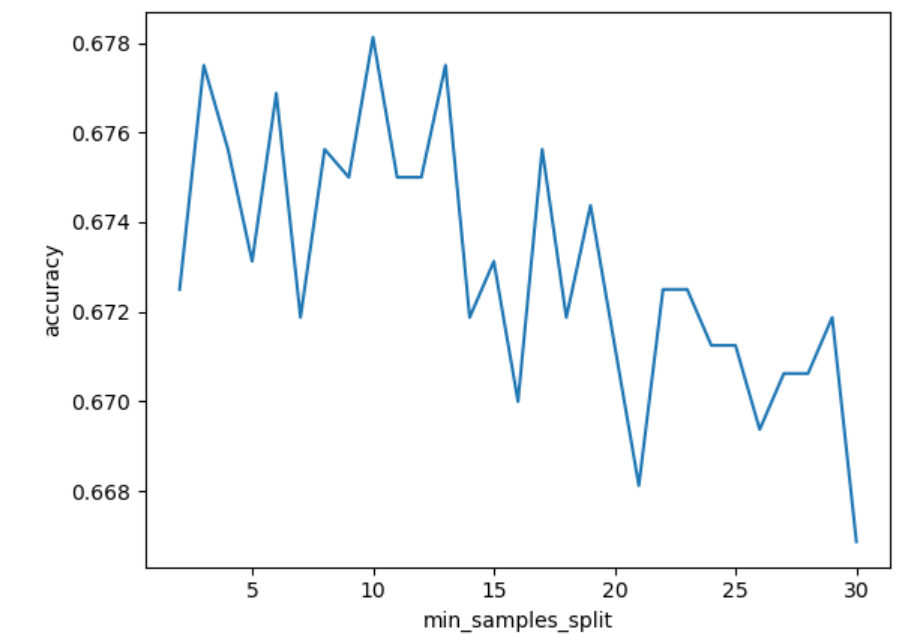
\includegraphics[width=0.3\linewidth]{image7.png}
    %\caption{Enter Caption}
    \label{fig:enter-label}
% \end{figure}
% \begin{figure}
    \righting
    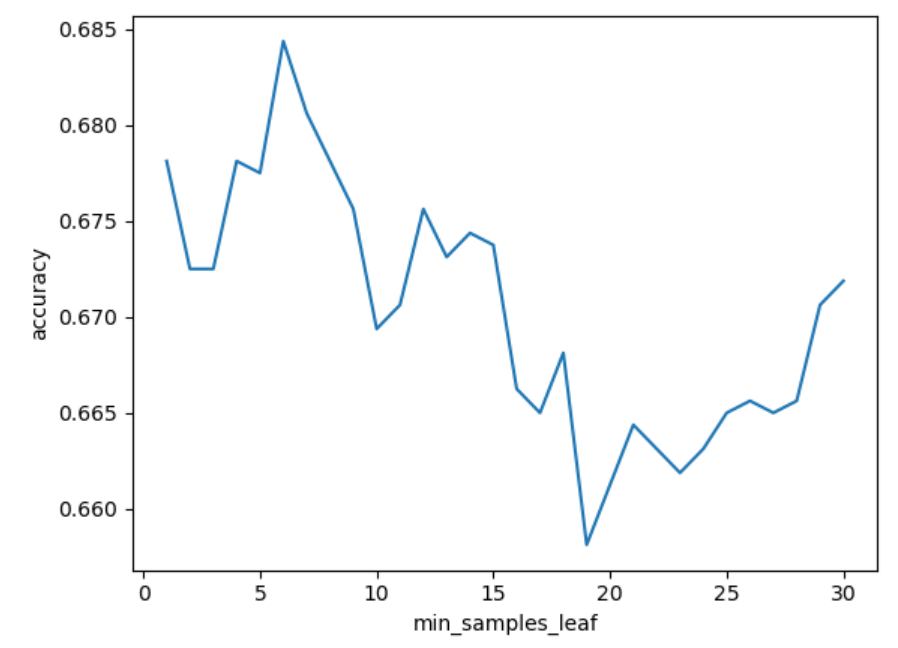
\includegraphics[width=0.3\linewidth]{image8.png}
    % \caption{Enter Caption}
    \label{fig:enter-label}
\end{figure}

所以,我们把\lstinline|max_depth|的范围设置为$5$—$10$,\lstinline|min_samples_split|的范围设置为$2$—$15$,\lstinline|min_samples_leaf|的范围设置为$2$—$6$,并找出最优的参数组合。最终,这个最优超参数组合在验证集上的结果是
\begin{figure}[h]
    \centering
    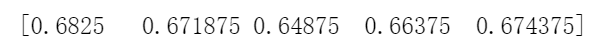
\includegraphics[width=0.5\linewidth]{image9.png}
    %\caption{Enter Caption}
    \label{fig:enter-label}
\end{figure}
\newpage

\subsubsection{多层感知机}
多层感知机实际上是一种人工神经网络,由多个节点层组成,每一层的节点都全连接到下一层。相比于前面几个模型,多层感知机更加强大,适用于文本数据集这种复杂的数据集。

为了尽可能得到更高的正确率,我们把迭代次数、层数和每一层的神经元数都设置得大一些,分别为$5000$、$100$和$100$。本来想要调整一下每一批的大小\lstinline|batch_size|,但是在实验后发现实际上这个超参数对准确率并没有什么影响。
\begin{figure}[h]
    \centering
    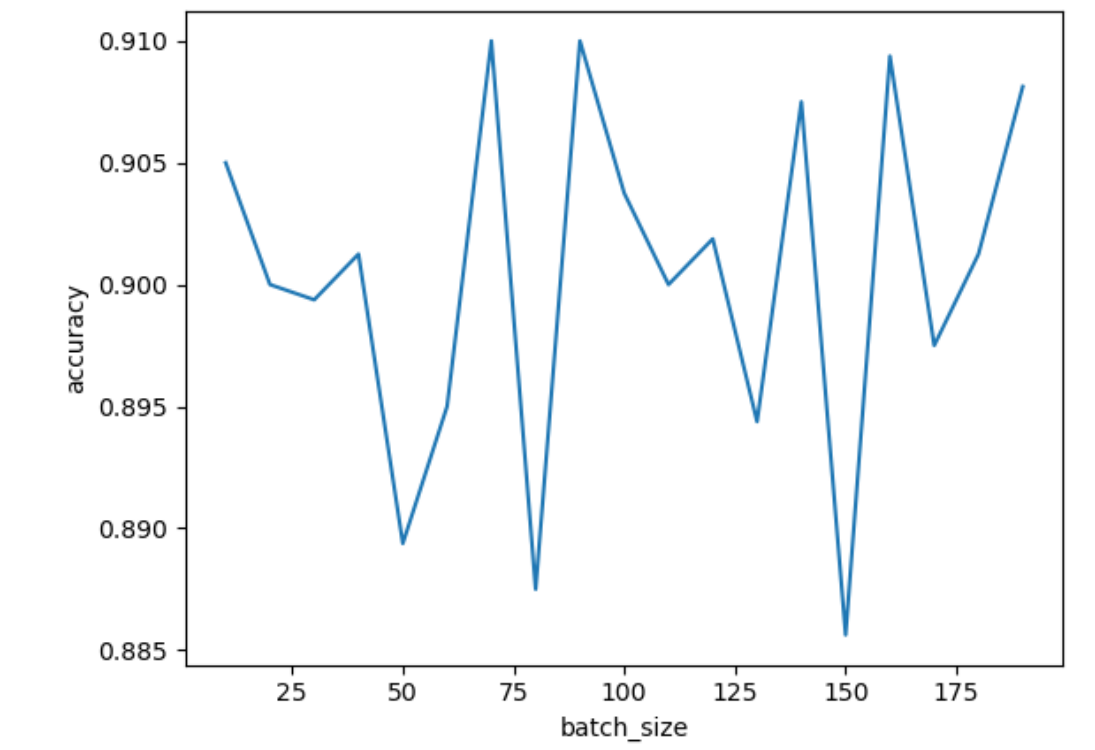
\includegraphics[width=0.5\linewidth]{image10.png}
    %\caption{Enter Caption}
    \label{fig:enter-label}
\end{figure}

所以,我们干脆不管这个参数,把它设置为默认值。接下来,尝试权重优化方式\lstinline|solver|和是否早停\lstinline|early_stopping|的各种组合,并把最优组合设置为超参数进行五折交叉验证,得到的准确率为
\begin{figure}[h]
    \centering
    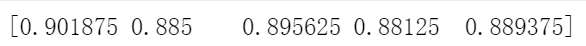
\includegraphics[width=0.5\linewidth]{image11.png}
    %\caption{Enter Caption}
    \label{fig:enter-label}
\end{figure}

\subsubsection{textRNN}
如果要使用更加复杂的深度学习模型来完成这个文本分类任务,可以考虑textCNN、textRNN和Bert。这里发生了一个小插曲。我在选择模型时,本来打算用Bert,因为它的调用接口看起来更加简洁好用,训练前对于数据处理的要求也更低。但是Bert这个模型占据的空间太大了,以至于在运行的时候内存崩了。在助教的指导下,我在colab上进行了实验,但没想到colab的T4 GPU也无法支撑哪怕是像DistilBert这样更加轻量化的Bert模型。于是我便考虑使用textCNN或者textRNN。查阅资料后我发现,RNN最早就是为了文本分类才设计出来的,而CNN起初是用来进行图像分类的。所以,我选择使用textRNN来进行文本分类。

RNN的中文名叫“循环神经网络”。有别于传统的神经网络,循环神经网络从先前的输入中获取信息,以影响当前的输入和输出。具体到文本分类,神经网络会根据当前的几个单词的位置来预测下一个单词。这么看,RNN同样是通过利用上下文信息来提升分类的准确度。

在训练之前,我们还需要对初始的文本进行一些加工。我们要对文本进行分词,并将所有文本统一为同一个长度:短于这个长度的文本需要用空格补齐,长于这个长度的文本会被截断。
\begin{lstlisting}
# 将文本转换为序列
X_train = tokenizer.texts_to_sequences(train_df['raw'])
X_val = tokenizer.texts_to_sequences(val_df['raw'])
# 填充序列,使它们具有相同的长度
max_length = 128  # 最大长度
X_train = pad_sequences(X_train, maxlen=max_length, padding='post')
X_val = pad_sequences(X_val, maxlen=max_length, padding='post')
\end{lstlisting}
处理完原始数据后,我们仍旧把处理后的数据集按照$2:8$的比例划分为训练集和验证集。在设置超参数时,为了在控制训练时间的同时让准确率尽可能高,我们把迭代次数设置为$75$轮。可以看到,在进行了$75$轮迭代后,模型在验证集上的准确率超过了$99\%$。
\begin{figure}[h]
    \centering
    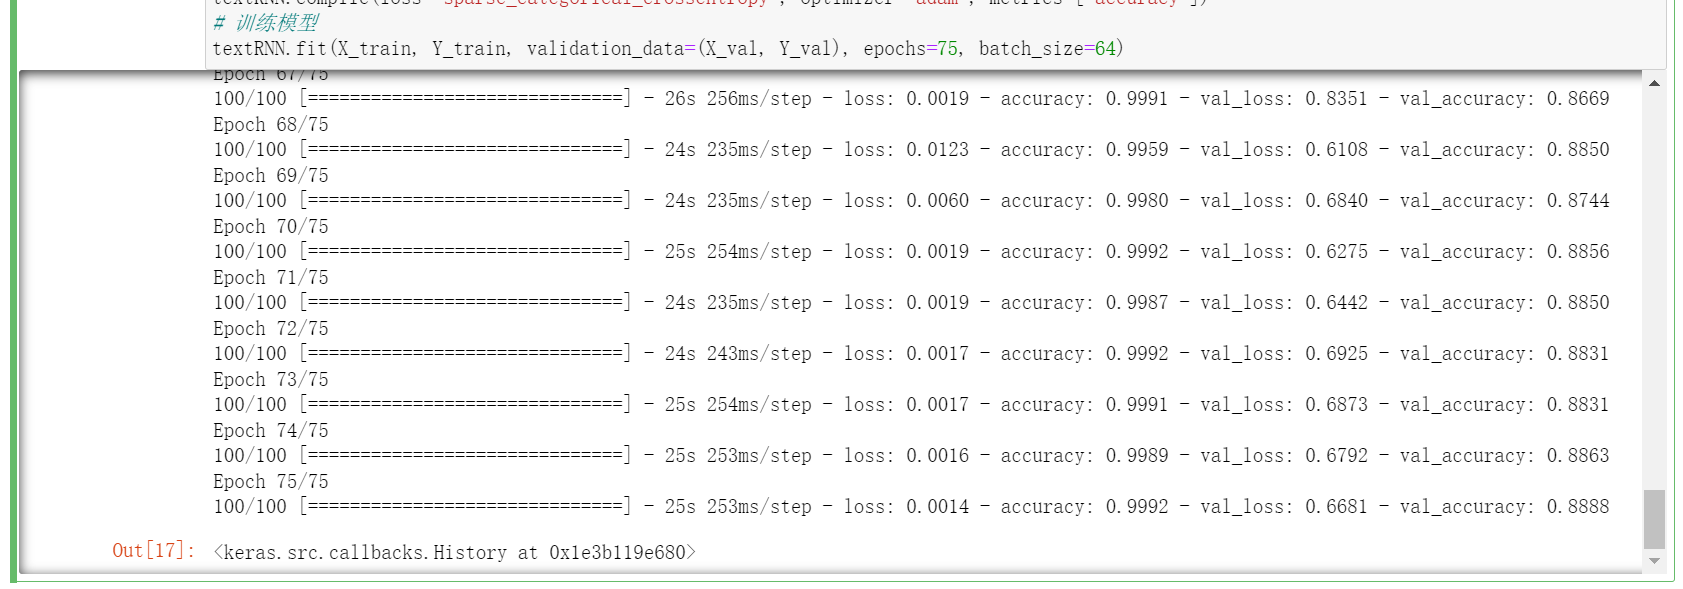
\includegraphics[width=\linewidth]{image12.png}
    %\caption{Enter Caption}
    \label{fig:enter-label}
\end{figure}

\subsection{模型测试}
从上面的实验结果来看,textRNN的准确率最高,所以最后提交的测试集分类结果\lstinline|./results.txt|也是textRNN模型生成的。
\begin{lstlisting}
X_test_hand_in = tokenizer.texts_to_sequences(ft['text'])
X_test_hand_in = pad_sequences(X_test_hand_in, maxlen=max_length, padding='post')
preds = textRNN.predict(X_test_hand_in)
test_ids = ft.index
results_df = pd.DataFrame({'id': test_ids, 'pred': preds.argmax(axis=1)})
with open("results.txt", "w") as file:
    file.write('id, pred\n')
    for i in range(len(results_df)):
        cur_id=results_df['id'][i]
        cur_pred=results_df['pred'][i]
        file.write(f'{cur_id}, {cur_pred}\n')
\end{lstlisting}
\begin{figure}[h]
    \centering
    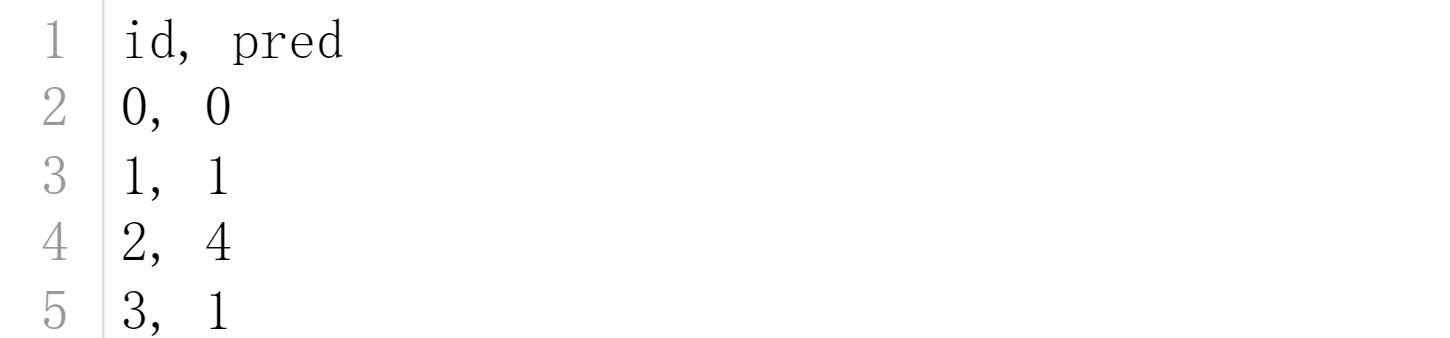
\includegraphics[width=1\linewidth]{image13.png}
    %\caption{Enter Caption}
    \label{fig:enter-label}
\end{figure}
\section{结果分析与讨论}
实验结果中有两个值得注意的点。

第一点是,为什么其他模型的准确率都能在调参后达到接近$0.9$甚至$0.9$以上的准确率,而决策树的准确率无论如何也无法超过$0.7$。决策树是通过自变量(在本实验中是文本)的取值来逐层进行分类的,而文本数据特征过于复杂,又是非线性数据集,导致决策树在文本数据集上表现不佳。此外,在训练决策树时,如何剪枝、如何控制树的深度是个很复杂的问题。如果树的最大深度设置得过小,会导致欠拟合,反之亦然。相比之下,另外四个模型在面对文本数据这种复杂的、非线性的数据集时表现更好。

第二点是,同样是神经网络,多层感知机的准确率再怎么调参也超不过$0.91$,但textRNN的准确率却能达到$0.99$。首先,在前面已经提到,textRNN能够捕捉文本中的序列信息和上下文关系,从而能够更好地处理自然语言的语义和结构;相比之下,多层感知机是一种前馈神经网络,不擅长捕捉文本中的序列信息,所以在文本分类任务中表现更差。此外,在训练textRNN时,我们并没有使用预先生成的文本向量,仅仅是对文本进行分词、长度对齐就把文本数据喂给模型,让模型直接从文本中通过学习提取特征。相比之下,多层感知机往往需要手动设计或选择适当的特征表示。


\section{总结}
在本次实验中,我们第一次经历了数据预处理、模型选择、调参、训练、交叉验证等人工智能的大致工作流程,为以后的学习和实践打好了基础。本次实验中,囿于时间的限制,我没能尝试更多的参数组合,也没有加大迭代次数,否则还能得到更高的准确率。另外,对于那些比较复杂的深度学习模型,我也没有比较深刻的理解,所以对于不同模型准确率高低的原因的分析还不够到位。这些都要在后面三个月的课程学习当中补足。


\begin{thebibliography}{99}  

\bibitem{ref1}\href{https://zhuanlan.zhihu.com/p/103136609}{机器学习超详细实践攻略(9):决策树算法使用及小白都能看懂的调参指南}

\end{thebibliography}

\end{document}